%%%%%%%%%%%%%%%%%%%%%%%%%%%%%%%%
% Title: Notes of Intermediate Microeconomic                           %                 
% Author: GANG LI                                                                    %
% Institute: Department of Business Administration,                 %
%                Zhongnan University of Economics and Law         %
% Email: gang.li@stu.zuel.edu.cn                                             %
% Github: GangLi-0814                                                             %
%%%%%%%%%%%%%%%%%%%%%%%%%%%%%%%%

\documentclass[UTF8]{ctexbeamer}

\usetheme{CambridgeUS}
\usecolortheme{default} 

\usepackage{graphicx}
\usepackage{animate}
\usepackage{color}
\usepackage{hyperref}
%\usepackage{hyperref}
%\hypersetup{
%    colorlinks=true,
%    linkcolor=blue,
%    filecolor=blue, 
%    urlcolor=blue,
%    citecolor=cyan,
%}
\usepackage{tikz}
\usetikzlibrary{decorations.pathreplacing}
\usepackage{amsmath} % 公式
\usepackage{booktabs} %表格框线
\usepackage{xcolor}
\usepackage{multirow}
\usepackage{setspace} % 调整行距
\setbeamertemplate{caption}[numbered] % 图形编号
\usepackage{threeparttable} % 表格添加注释
\usepackage{multicol} % 目录分栏

 % 设置字体
\usepackage{xeCJK}
\setCJKmainfont[BoldFont=STSongti-SC-Regular, ItalicFont=STSongti-SC-Regular]{STSongti-SC-Regular}
\setCJKsansfont[BoldFont=STSongti-SC-Regular]{STSongti-SC-Regular}
\setCJKmonofont{STSongti-SC-Regular}
\setmainfont{TimesNewRomanPSMT}  %英文字体


%%%%%%%%%%%%
% 封面
%%%%%%%%%%%%
\title{中级微观经济学笔记}
%\subtitle{\textit{A Powerful Tool for Reference Management}}
\author{李刚}
\institute{中南财经政法大学}
\date{\today}

\begin{document}

\frame{\titlepage} 

%%%%%%%%%%%%%%%%%
% 作者简介
%%%%%%%%%%%%%%%%
%\begin{frame}{作者简介}
%\begin{columns}
%\begin{column}{.3\linewidth}
%\begin{figure}
%\centering
%
\includegraphics[width=30mm]{figures/fig_0.jpg}
%\end{figure}
%\end{column}
%\begin{column}{.7\linewidth}
%\linespread{1.2}
%\scriptsize
%\begin{itemize}
%\item 李刚,中南财经政法大学工商管理学院硕士研究生,导师为陈池波教授,研究方向为农业经济理论与政策。在校期间,主持完成中央高校基本科研业务费项目1项,参与联合国开发计划署与商务部中国经济技术交流中心合作项目1项;在《农业技术经济》(二作、通讯作者)上发表论文1篇,会议论文获湖北省第三届乡村振兴高峰论坛二等奖;2019-2020学年研究生学业奖学金一等奖、国家奖学金获得者。
%\item 擅长Stata和Python等工具,曾先后在北京大学中国家庭追踪调查(CFPS)项目组、北京大学中国教育财政科学研究所(CIEFR)农村教育课题组和清华大学中国工程科技发展战略研究院(CIEDS)从事数据处理与分析工作,熟悉常用的企业层面数据库和微观调查数据库。
%\item 联系方式:邮箱(\href{mailto:gang.li@stu.zuel.edu.cn}{gang.li@stu.zuel.edu.cn})、微信公众号(\href{http://lgspace.top/2020/11/23/resume/}{PyStaData})、个人博客(\href{http://lgspace.top}{http://lgspace.top})。
%\end{itemize}
%\end{column}
%\end{columns}
%\end{frame}


%%%%%%%%%%%%
% 大纲
%%%%%%%%%%%%
%% 显示为 1 列
%\begin{frame}{大纲}
%  \tableofcontents
%\end{frame}

% 大纲显示为 2 列
\begin{frame}{大纲}
\begin{multicols}{2}
  \tableofcontents
\end{multicols}
\end{frame}

%% 在每节前显示大纲
%\AtBeginSection[]{
%    \frame{\frametitle{大纲}
%    \begin{multicols}{2}
%    \tableofcontents[sectionstyle=show/shaded,subsectionstyle=show/show/shaded]
%      \end{multicols}
%        }
%}

%%%%%%%%%%%%%%%
% 第一篇 市场和价格
%%%%%%%%%%%%%%%
\section{市场和价格}

\subsection{绪论}
\begin{frame}{绪论}
\begin{block}{微观经济学}
经济学的分支,主要研究个体经济单位——消费者、厂商、工人和投资者的行为,以及由这些个体组成的市场本身的行为。

微观经济学以消费者和生产者的决策行为为研究重点,探讨在不同的市场结构下生产者的决策和市场均衡等问题。其内容主要包括消费者的效用最大化问题,生产者的成本最小化和利润最大化问题,厂商均衡理论、局部均衡和一般均衡理论等。

\end{block}
\begin{block}{宏观经济学}
经济学的分支,主要研究总量经济指标,诸如国民产出的水平和增长率、利率、失业以及通货膨胀。
\end{block}
\end{frame}

\subsection{供求理论}
\begin{frame}{供求理论}
\linespread{1.5}
\begin{itemize}
\item 供给和需求
\item 市场均衡及其变动
\item 弹性
\end{itemize}
\end{frame}

\subsubsection{供给和需求}
\begin{frame}{供给}
\begin{block}{供给曲线}
描绘生产者愿意出售的商品数量与该商品价格之间关系的曲线。\newline 用方程表示为:
\begin{equation*}
Q_s = Q_s(P) 
\end{equation*}   
\end{block}

供给的变动(change in supply):供给对于其他变量变动的反应,如厂商的生产成本(工资、利息和原材料的成本)。  \newline
供给量的变动(change in the quantity supplied):供给量随价格的变化而发生变化的过程,表现为沿着供给曲线的移动。
\end{frame}


\begin{frame}{需求}
\begin{block}{需求曲线}
消费者愿意购买的数量和该商品价格之间的关系。\newline 用方程表示为:
\begin{equation*}
Q_d = Q_d(P)
\end{equation*}
\end{block}
影响商品需求的因素:季节转换(如燃料、雨衣和雨伞等)、相关商品的价格变动(如石油价格的上升导致天然气需求增加)、消费者口味变化等 \newline

注意区分:{\heiti 需求的变动}和{\heiti 需求量的变动}
\end{frame}

\begin{frame}{供需理论的应用}
\linespread{1.5}
当描绘和使用供给和需求曲线时,假定在任一给定的价格下,一个给定的商品数量被生产和出售。这一假设在市场至少大体上是竞争性的情况下才被满足。如果有垄断的存在,价格和供给量就不是一一对应的关系。\newline
因此,{\heiti 运用供给曲线和需求曲线时,一个隐含的假定时分析对象是竞争性市场。}
\end{frame}

\subsubsection{均衡及其变动}
\begin{frame}{均衡及其变动}
\linespread{1.5}
\begin{itemize}
\item 供给变动后的新均衡
\item 需求变动后的新均衡
\item 供给和需求变动后的新均衡
\end{itemize}
价格和数量的变化取决于供给曲线和需求曲线的移动幅度以及曲线的形状。要预测这类变化的大小和方向,必须要能够定量地分析供给和需求对价格和其他变量的依赖程度(弹性)。
\end{frame}

\begin{frame}{均衡及其变动}
\begin{figure}
\centering
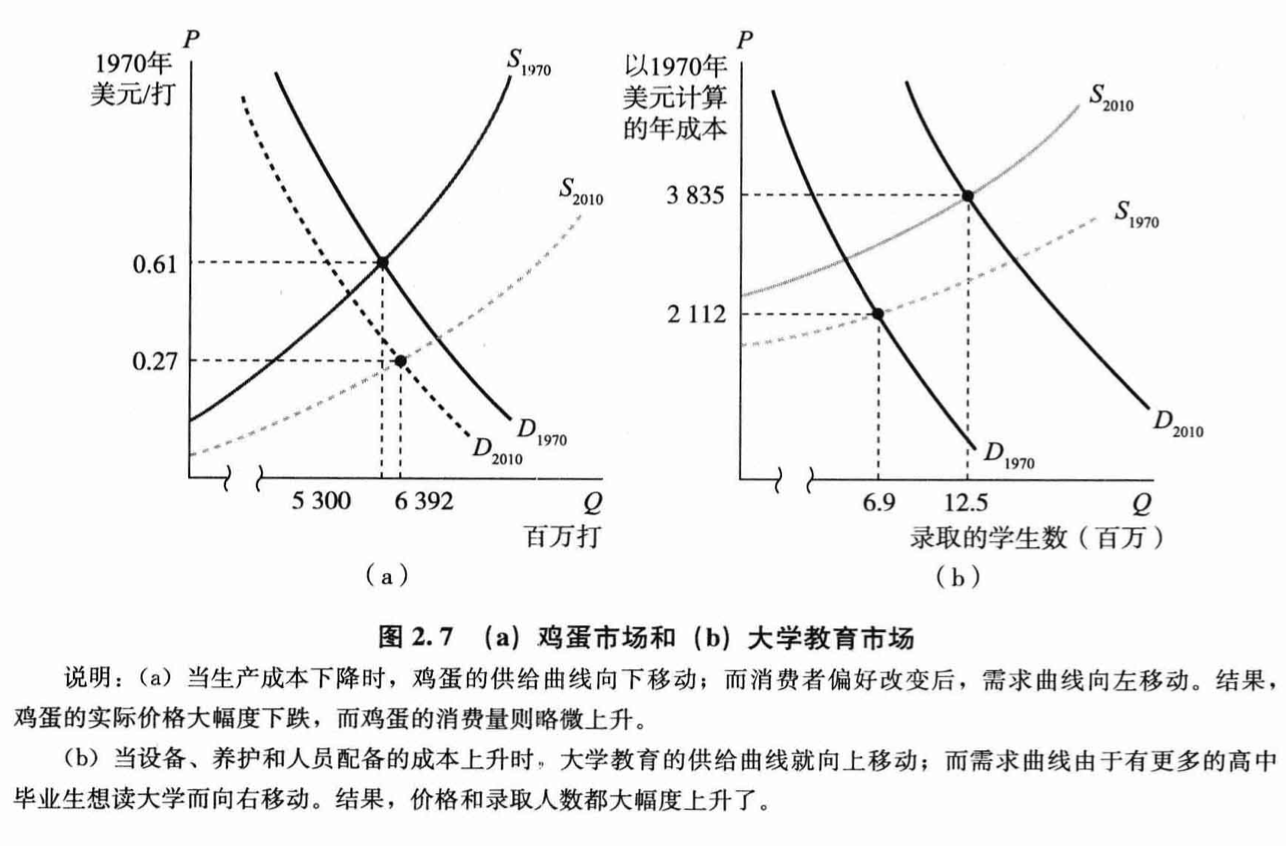
\includegraphics[width=110mm]{figures/2_1.png}
\end{figure}
\end{frame}

\subsubsection{弹性理论}
\begin{frame}{弹性}
\begin{block}{弹性}
某一变量变动 $ 1\% $ 所引起的另一变量变动的百分比。
\end{block}
\begin{block}{需求的价格弹性}
商品价格上升 $ 1\% $ 所导致的的需求量变动的百分比。用公式表示为:
\begin{equation*}
E_p = \frac{\Delta Q / Q}{\Delta P / P} = \frac{P\Delta Q}{Q\Delta P}
\end{equation*}
\end{block}
\begin{block}{需求的收入弹性}
由于收入上升 $ 1\% $ 所导致的的需求量变动的百分比。
\end{block}
\begin{block}{需求的交叉价格弹性}
某一种商品价格增加 $ 1\% $ 所导致的的需求量变动的百分比。
\end{block}
\end{frame}

\begin{frame}{短期弹性与长期弹性}
\linespread{1.5}
当分析需求与供给时,必须区分长期和短期。在长期中,消费者和生产者有足够的时间来充分调整以适应价格的变动。
\begin{itemize}
\item 消费习惯
\item 耐用性
\item 周期性行业
\end{itemize}
\end{frame}

\begin{frame}{价格控制}
\linespread{1.5}
\begin{itemize}
\item 最高限价
\item 最低限价
\end{itemize}
\end{frame}

%%%%%%%%%%%%%%%%%%%%%
% 第二篇 生产者、消费者与竞争性市场
%%%%%%%%%%%%%%%%%%%%%
\section{生产者、消费者与竞争性市场}

\subsection{消费者行为理论}
\begin{frame}{消费者行为}
\begin{itemize}
\item 消费者偏好
\item 预算约束
\item 消费者选择
\item 显示偏好
\item 边际效用与消费者选择
\item 生活成本指数
\end{itemize}
\end{frame}

\subsubsection{消费者偏好}
\begin{frame}{消费者偏好}
\begin{itemize}
\item 偏好及其假设
\item 无差异曲线
\item 边际替代率
\item 效用
\end{itemize}
\end{frame}

\subsubsection{预算约束}
\begin{frame}{预算约束}
\begin{itemize}
\item 预算线及其变动
\end{itemize}
\end{frame}

\subsubsection{消费者选择}
\begin{frame}{消费者选择}
\linespread{1.5}
消费者的最优选择是:在给定的有限预算下,选择能带来最大满足的商品组合。
\begin{enumerate}
\item 必须位于预算线上
\item 必须能给予消费者其最偏好的商品和服务组合
\end{enumerate}
\end{frame}

\subsubsection{显示偏好}
\begin{frame}{显示偏好}
\end{frame}

\subsubsection{生活成本指数}
\begin{frame}{生活成本指数}
\begin{block}{拉氏指数}
以当期价格购买一个{\heiti 基期选定}的商品或服务组合所需的货币数除以基期价格购买同一组合所需的货币数之和。
\end{block}

\begin{block}{帕氏指数}
以当期价格购买一个{\heiti 当期选定}的商品或服务组合的购买成本与以基期价格购买同一组合的购买成本之比。
\end{block}
\end{frame}

\subsubsection{不确定性与消费行为}
\begin{frame}{不确定性与消费行为}
\begin{itemize}
\item 描述风险
\end{itemize}
\end{frame}

\subsection{个人需求和市场需求}
\begin{frame}{个人需求和市场需求}
\begin{itemize}
\item 收入效应与替代效应
\item 正常品与劣等品
\item 恩格尔曲线
\item 消费者剩余
\item 网络外部性
\end{itemize}
\end{frame}


\subsection{生产者理论}
\begin{frame}{生产者理论}
\begin{itemize}
\item 厂商及其生产决策
\item 一种可变投入(劳动)下的生产
\item 两种可变投入下的生产
\item 规模报酬
\end{itemize}
\end{frame}

%%%%%%%%%%%%%%%%%%%%%
% 第三篇 市场结构与竞争策略
%%%%%%%%%%%%%%%%%%%%%
\section{市场结构与竞争策略}

\subsection{市场结构}
\begin{frame}{市场结构}
\begin{itemize}
\item 垄断
\item 有市场势力的定价
\item 垄断竞争和寡头垄断
\end{itemize}
\end{frame}


\subsection{竞争策略}
\begin{frame}{竞争策略}
\begin{itemize}
\item 博弈论
\end{itemize}
\end{frame}

%%%%%%%%%%%%%%%%%%%%%
% 第四篇 信息、市场失灵与政府角色
%%%%%%%%%%%%%%%%%%%%%
\section{ 信息、市场失灵与政府角色}

\subsection{一般均衡与经济效率}
\begin{frame}{一般均衡与经济效率}
\end{frame}


\subsection{信息不对称的市场}
\begin{frame}{信息不对称的市场}
\end{frame}

\subsection{外部性与公共物品}
\begin{frame}{外部性与公共物品}
\end{frame}


%%%%%%%%%
% 联系方式
%%%%%%%%%
%\begin{frame}
% \begin{center}
%{\huge \emph{\textcolor{blue}{Thank  ~you!}}}\\
%\vspace{5mm}\large
%\begin{tabular}{ll}
%{\sc Author}:  & GANG Li\\
%{\sc Address}: &Department of Business Administration\\
%               & Zhongnan University of Economics and Law\\
%               & Wuhan, 430073, China\\
%  {\sc Email}: & \href{mailto:gang.li@stu.zuel.edu.cn}{\color{blue}gang.li@stu.zuel.edu.cn}\\
%\end{tabular}
%\end{center}
%\end{frame}

\begin{frame}{联系方式}
\begin{columns}
\begin{column}{.4\linewidth}
\begin{figure}

\includegraphics[width=40mm]{figures/Wechat_QR.jpeg}
\end{figure}
\end{column}
\begin{column}{.6\linewidth}
{\huge \emph{\textcolor{blue}{Thank  ~you!}}}\\
\vspace{5mm}\large
\begin{tabular}{ll}
{\sc Author}:  & GANG Li\\
{\sc Github}: & \href{https://github.com/GangLi-0814}{\color{blue}{GangLi-0814}}\\
{\sc Blog}: & \href{http://lgspace.top}{\color{blue}http://lgspace.top}\\
{\sc Email}: & \href{mailto:gang.li@stu.zuel.edu.cn}{\color{blue}gang.li@stu.zuel.edu.cn}\\
\end{tabular}
\end{column}
\end{columns}
\end{frame}


\end{document}


